\subsection*{Pruning algorithm}
Computer vision techniques were increasingly being used in computer graphics to create image-based models of real-world objects, to create visual effects, and to merge realworld imagery using computational photography techniques. Our decision to focus on the applications of computer vision to fun problems such as image stitching and photo-based 3D modeling from personal photos. \cite{ref11}

The example of such neural network , Pruning algorithm, which is the process of removing connections (and neurons) from a neural network while preserving its functionality, the goal is to reduce the storage and energy required to run inference on such large networks so they can be deployed on mobile devices, it can also can reduce network complexity and over-fitting, As shown on the left side of Figure 1, we start by learning the connectivity via normal network training. Next, we prune the small-weight connections: all connections with weights below a threshold are removed from the network \cite{ref22}

	\begin{figure}[h]
		\centering
		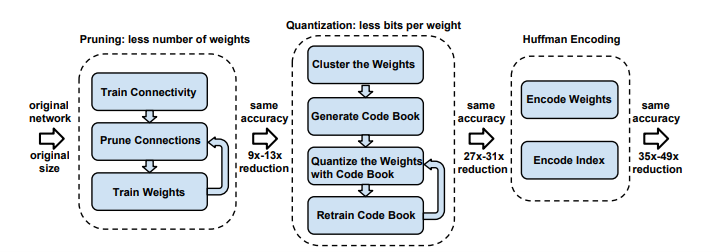
\includegraphics[width=0.5\textwidth]{section/images/Picture1.png}
		
		\label{fig:labelname}
	\end{figure}
Also, Pruning typically proceeds by training the original network, removing connections, and further fine-tuning. \cite{ref33} 
	
\subsection*{Experience of Pruning algorithm}
We test our pruning scheme on the large-scale ImageNet classification task. In the first experiment, we begin with a trained CaffeNet implementation of AlexNet with 79.2\% top-5 validation accuracy. Between pruning iterations, we fine-tune with learning rate $10^{-4}$ , momentum 0.9, weight decay $10^{-4}$, batch size 32, and drop-out 50\%. Using a subset of 5000 training images, we compute oracle-abs and Spearman’s rank correlation with the criteria, as shown in Table 1. Pruning traces are illustrated in Fig.1 .\cite{ref44} 
	\begin{figure}[h]
	\centering
	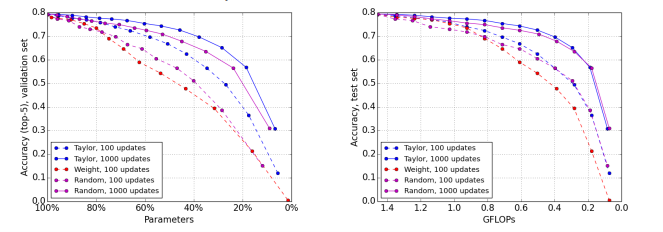
\includegraphics[width=0.5\textwidth]{section/images/Picture2.png}
	\caption{Pruning of AlexNet on Imagenet with varying number of updates between pruning iterations.}
	\label{fig:labelname}
\end{figure}
\subsection*{The limitations of the pruning algorithm}
The pruning algorithm has certain limitations, including loss of precision, sensitivity to initialization, the need for retraining the model, reduced interpretability, dependence on the model and data, complexity of pruning techniques, and its impact on online learning. It is important to consider these limitations when using the pruning algorithm and to choose appropriate parameters and techniques based on the specific use case.
\subsection*{Application of Pruning algorithm in Mobile application}
One example of pruning algorithm in mobile application is the work done by Sze et al. (2017) where they proposed a framework called "MobileNets" which utilizes depthwise separable convolutions for mobile vision applications. Depthwise separable convolutions separate the spatial and channelwise convolutions into two separate layers, which greatly reduces the number of parameters and computational complexity of the neural network.

Additionally, the MobileNets framework also utilizes pruning to remove unnecessary channels and parameters, further reducing the size and computational cost of the model. The authors showed that their framework achieved state-of-the-art accuracy on several mobile vision benchmarks while being up to 32 times smaller than other state-of-the-art models. \cite{ref55}


%------------------------------------------------